%%%%%%%%%%%%%%%%%%%%%%%%%%%%%%%%%%%%%%%%%
% a0poster Portrait Poster
% LaTeX Template
% Version 1.0 (22/06/13)
%
% The a0poster class was created by:
% Gerlinde Kettl and Matthias Weiser (tex@kettl.de)
% 
% This template has been downloaded from:
% http://www.LaTeXTemplates.com
%
% License:
% CC BY-NC-SA 3.0 (http://creativecommons.org/licenses/by-nc-sa/3.0/)
%
%%%%%%%%%%%%%%%%%%%%%%%%%%%%%%%%%%%%%%%%%

%----------------------------------------------------------------------------------------
%	PACKAGES AND OTHER DOCUMENT CONFIGURATIONS
%----------------------------------------------------------------------------------------

\documentclass[a0,portrait]{a0poster}

\usepackage{multicol} % This is so we can have multiple columns of text side-by-side
\columnsep=100pt % This is the amount of white space between the columns in the poster
\columnseprule=3pt % This is the thickness of the black line between the columns in the poster

\usepackage[svgnames]{xcolor} % Specify colors by their 'svgnames', for a full list of all colors available see here: http://www.latextemplates.com/svgnames-colors

\usepackage{times} % Use the times font
%\usepackage{palatino} % Uncomment to use the Palatino font

\usepackage{graphicx} % Required for including images
\usepackage{booktabs} % Top and bottom rules for table
\usepackage[font=small,labelfont=bf]{caption} % Required for specifying captions to tables and figures
\usepackage{amsfonts, amsmath, amsthm, amssymb} % For math fonts, symbols and environments
\usepackage{wrapfig} % Allows wrapping text around tables and figures
\usepackage{url}

\begin{document}

%----------------------------------------------------------------------------------------
%	POSTER HEADER 
%----------------------------------------------------------------------------------------

% The header is divided into two boxes:
% The first is 75% wide and houses the title, subtitle, names, university/organization and contact information
% The second is 25% wide and houses a logo for your university/organization or a photo of you
% The widths of these boxes can be easily edited to accommodate your content as you see fit

\begin{minipage}[b]{0.75\linewidth}
\veryHuge \color{NavyBlue} \textbf{RADISH: The System Balance of Power for Large Data Centers} \color{Black}\\ % Title
\Huge\textit{Evaluating Amdahl's Rule of Thumb with Google Cluster Data}\\[2cm] % Subtitle
\huge \textbf{Vincent Lee \& Shumo Chu}\\[0.5cm] % Author(s)
\huge University of Washington: Computer Science and Engineering\\[0.4cm] % University/organization
\end{minipage}
%
\begin{minipage}[b]{0.25\linewidth}

\includegraphics[width=20cm]{cse_logo.png}\\
\end{minipage}

\vspace{1cm} % A bit of extra whitespace between the header and poster content

%----------------------------------------------------------------------------------------

\begin{multicols}{2} % This is how many columns your poster will be broken into, a portrait poster is generally split into 2 columns

%----------------------------------------------------------------------------------------
%	ABSTRACT
%----------------------------------------------------------------------------------------

\color{Navy} % Navy color for the abstract

\section{Introduciton}

The design of large data centers is driven by application workloads, performance targets, energy efficient constraints, and system scalability.
To build these systems, we rely on empirical analysis and engineering intuition to properly allocate the amount of computation, memory, disk, and networking I/O to satisfy these contraints.
A system with insufficient resources will perform poorly as a single component of the system can bottleneck progress.
Alternatively, a system with over-provisioned resources is wasteful and can expend unnecessary energy and silicon area.
Ideally, we'd like to construct systems which have sufficient amounts of memory, compute, disk, and network I/O but at the same time not overprovision these resources.

%----------------------------------------------------------------------------------------
%	INTRODUCTION
%----------------------------------------------------------------------------------------

\color{SaddleBrown} % SaddleBrown color for the introduction

\section*{Amdahl's Rules of Thumb for a Balanced System}

Amdahl's Rules of Thumb for a balanced system proposed in ~\cite{export:68636, Bell:2006:PCS:1110638.1110681} suggest that an ideally balanced system roughly adhere to the following ratios:
\begin{enumerate}
\item Amdahl's parallelism law: if a computation has serial component S and parallel component P, then the maximum speedup is (S+P)/S
\item Amdahl's balanced system law: a system needs one bit of memory IO per second for each instruction per second
\item Amdahl's memory law: in a balanced system, the ratio $\alpha$ of the size of memory in MB to the instructions per second in million instructions per second (MIPS) is 1 MB per 1 MIPS or $\alpha = 1$
\item Amdahl's IO law: programs do one memory IO per 50000 instructions
\end{enumerate}

%----------------------------------------------------------------------------------------
%	OBJECTIVES
%----------------------------------------------------------------------------------------

\color{DarkSlateGray} % DarkSlateGray color for the rest of the content

\section*{Main Objectives}

We seek to analyze the publically available Google Cluster Data trace described in ~\cite{clusterdata:Reiss2011}.
The Google Cluster Data trace consists of job and task usage measurements recorded over a period of 29 days in May of 2009 at an undisclosed data center. 
Using the data trace, we seek to:

\begin{enumerate}
\item[1] Determine if it is possible to extract meaningful system balance ratios between compute, memory, disk, and networking I/O using the obfuscated traces, even order of magnitude calculations are sufficient.
\item[2] Determine what insights if any, these system balance ratios provide with respect to Amdahl's Rules of Thumb.
\end{enumerate}

We focus our attention on the task\_usage and task\_events traces which contain task granularity resource request quanities and actual usage records.

\begin{figure}
\centering
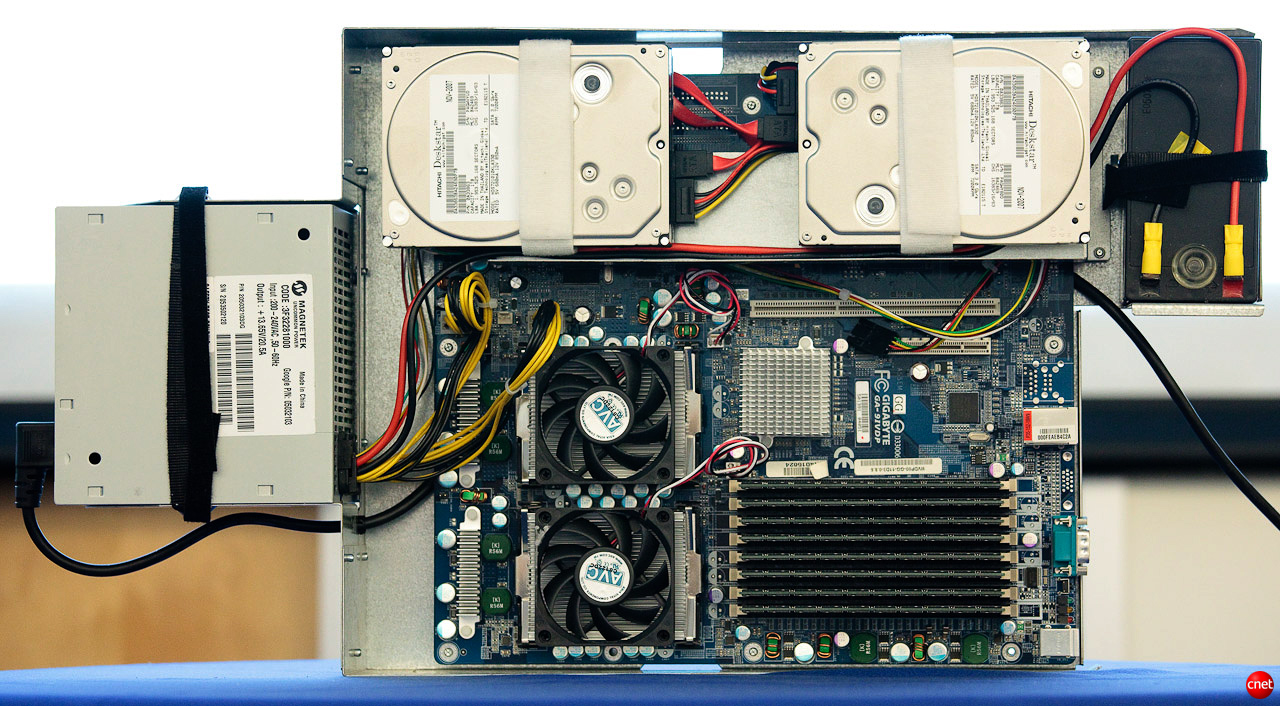
\includegraphics{GoogleServerLarge.jpg}
\label{google_server}
\caption{Google server motherboard and components unveiled in 2009 as described in ~\cite{googlehw}}
\end{figure}

%----------------------------------------------------------------------------------------
%	Google Cluster Trace
%----------------------------------------------------------------------------------------

\section*{Trace Obfuscation and Anamolies}

In order to protect details about the cluster parameters, the cluster traces were obfuscated before publishing.
Text fields were randomly hashed and numerical fields were normalized out of the largest value that appears in the trace.
In fact the obfuscation techniques were probably intended to counter a project such as this. 
Ideally, we'd like to compute exact system balance ratios, but an order of magnitude calculation is still possible and by no means meaningless. 
However, we can make reasonable order of magnitude estimates of the normalization factors, especially for system components such as RAM and CPU instructions per second. \\

Some trace entries were also missing from their records.
In ~\cite{clusterdata:Reiss2011}, these anamolies are attributed to bugs in the profiling infrastructure, and high system load which may cause diagnostic traffic to be lost.
We address these anamolies by cleaning the dataset and omitting their entries from the analysis where appropriate.

%----------------------------------------------------------------------------------------
%	RESULTS 
%----------------------------------------------------------------------------------------

\section*{Results}



RESULTS

%----------------------------------------------------------------------------------------
%	CONCLUSIONS
%----------------------------------------------------------------------------------------

\color{SaddleBrown} % SaddleBrown color for the conclusions to make them stand out

\section*{Conclusions}

While we were not able to procure exact system balance ratios, our order of magnitude calculations still provide enough insight to re-evaluate Amdahl's Rules of Thumb:

\noindent \bf{Amdahl's Parallelism Law} - clearly continues to hold \\
\bf{Amdahl's Memory Law} - \\
\bf{Amdahl's Balanced System and IO Law} - \\



\color{DarkSlateGray} % Set the color back to DarkSlateGray for the rest of the content

%----------------------------------------------------------------------------------------
%	FORTHCOMING RESEARCH
%----------------------------------------------------------------------------------------

\section*{Future Directions}

FUTURE WORK?

 %----------------------------------------------------------------------------------------
%	REFERENCES
%----------------------------------------------------------------------------------------

%\nocite{*} % Print all references regardless of whether they were cited in the poster or not
\bibliographystyle{plain} % Plain referencing style
\bibliography{poster.bib} % Use the example bibliography file sample.bib

\end{multicols}
\end{document}
